\section{\Glsfmtlong{cnn}}
\label{sec.cnn}

En dépit d'être une architecture naturelle pour le traitement des séquences,
les \glspl{rnn} sont trop lents pour la majorité des cas d'utilisation pratiques.
Cela est dû à leur nature séquentielle qui à son tour, 
est due à leur utilisation de boucles de rétroaction (Voire Section~\ref{sec.rnn}).
Une architecture sans telles boucles (i.e une architecture d'\gls{ffn}) est donc préférable.

Les \glspl{cnn} sont une famille d'\glspl{ffn} typiquement utilisés en traitement d'images.
Ils ont été introduits par~\cite{Fukushima_1980} et popularisés par%
~\cite{LeCun_Boser_Denker_Henderson_Howard_Hubbard_Jackel_1989,Lecun_Bottou_Bengio_Haffner_1998}.
Les \glspl{cnn} atteignent des performances comparables à celles des \glspl{rnn} sans mémoire explicite.
Ils y parviennent en exploitant un outil mathématique appelé produit de \emph{convolution}%
~\cite{Calin_2020}.

Le produit de convolution de deux signaux \(f\) et \(g\) est le signal \(f \ast g\) donné par
\begin{equation}
    \label{eq.convolution}
    u \mapsto \int_\reals f(u-t)g(t)\diff{t}
\end{equation}
il s'agit d'une opération commune en probabilité, analyse fonctionnelle, 
traitement de signaux et traitement d'images~\cite{Barbe_Ledoux_2012,Oppenheim_Schafer_2013}.
À partir d'elle, une autre opération appelée \emph{l'inter-corrélation} est définie.
L'inter-corrélation de \(f\) et \(g\) est notée \(f\star g\).
Elle est définie par
\begin{equation}
    \label{eq.cros-corr}
    u \mapsto \int_\reals f(t)g(t-u)\diff{t} = (f \ast g^-)(u)
\end{equation}
ou \(g^- : t \mapsto g(-t)\).
Intuitivement, elle mesure la similarité entre les deux signaux en question.
Les \glspl{cnn} utilisent l'inter-corrélation à la place des applications linéaires quelconques d'un \gls{mlp}.
Une couche de convolution unidimensionnelle calcul donc la fonction suivante
\begin{equation}
    \label{eq.layer-conv1d}
    x \mapsto \phi\left(x\star w + b\right)
\end{equation}
ou \(x\) est l'entrée et \(w\) est le paramètre entraînable de la couche, aussi appelé son \emp{noyau}
(Voire Figure~\ref{fig.layer-conv1d}).

\begin{figure}[hbt]
    \begin{center}
        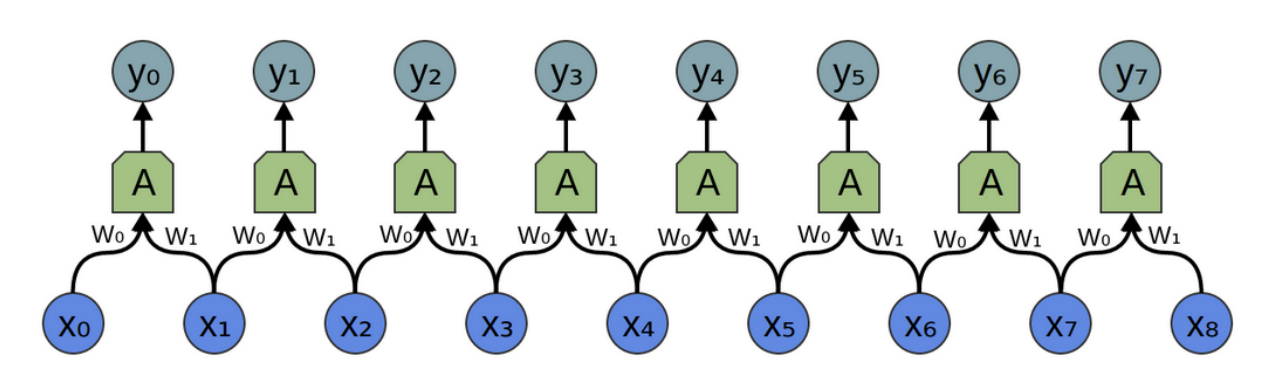
\includegraphics[width=\textwidth]{assets/images/conv1d.png}
    \end{center}    
    \caption{Une couche convolutive unidimensionnelle.}
    \label{fig.layer-conv1d}
\end{figure}